\documentclass[10pt,aspectratio=169]{beamer}
\usepackage[utf8]{inputenc}
\usepackage[T1]{fontenc}
\usepackage[french]{babel}
\usepackage{graphicx}
\usepackage{booktabs}
\usepackage{amsmath}
\usepackage{array}
\IfFileExists{commun/theme.tex}{\input{commun/theme.tex}}{%
  \IfFileExists{animation/commun/theme.tex}{\input{animation/commun/theme.tex}}{%
    \IfFileExists{theme_local.tex}{% Theme local de secours pour la presentation A9.
% Si un theme commun est fourni par le cours, le remplacer par ce fichier.
\usetheme{Madrid}
\usecolortheme{default}
\definecolor{espbleu}{RGB}{0,74,124}
\definecolor{esporange}{RGB}{197,90,17}
\definecolor{espvert}{RGB}{84,130,53}
\setbeamercolor{structure}{fg=espbleu}
\setbeamercolor{frametitle}{bg=espbleu,fg=white}
\setbeamercolor{title}{fg=espbleu}
\setbeamercolor{block title}{bg=espbleu,fg=white}
\setbeamercolor{block body}{bg=espbleu!5}
\setbeamertemplate{navigation symbols}{}
\setbeamertemplate{footline}{%
  \leavevmode%
  \hbox{%
    \begin{beamercolorbox}[wd=.72\paperwidth,ht=2.4ex,dp=1.2ex,leftskip=.3cm]{author in head/foot}%
      \usebeamerfont{author in head/foot}Groupe 3 --- A9 Consensus BFT
    \end{beamercolorbox}%
    \begin{beamercolorbox}[wd=.28\paperwidth,ht=2.4ex,dp=1.2ex,rightskip=.3cm plus1fil]{title in head/foot}%
      \usebeamerfont{title in head/foot}\insertframenumber/\inserttotalframenumber
    \end{beamercolorbox}%
  }%
  \vskip0pt%
}
}{%
      \IfFileExists{animation/theme_local.tex}{% Theme local de secours pour la presentation A9.
% Si un theme commun est fourni par le cours, le remplacer par ce fichier.
\usetheme{Madrid}
\usecolortheme{default}
\definecolor{espbleu}{RGB}{0,74,124}
\definecolor{esporange}{RGB}{197,90,17}
\definecolor{espvert}{RGB}{84,130,53}
\setbeamercolor{structure}{fg=espbleu}
\setbeamercolor{frametitle}{bg=espbleu,fg=white}
\setbeamercolor{title}{fg=espbleu}
\setbeamercolor{block title}{bg=espbleu,fg=white}
\setbeamercolor{block body}{bg=espbleu!5}
\setbeamertemplate{navigation symbols}{}
\setbeamertemplate{footline}{%
  \leavevmode%
  \hbox{%
    \begin{beamercolorbox}[wd=.72\paperwidth,ht=2.4ex,dp=1.2ex,leftskip=.3cm]{author in head/foot}%
      \usebeamerfont{author in head/foot}Groupe 3 --- A9 Consensus BFT
    \end{beamercolorbox}%
    \begin{beamercolorbox}[wd=.28\paperwidth,ht=2.4ex,dp=1.2ex,rightskip=.3cm plus1fil]{title in head/foot}%
      \usebeamerfont{title in head/foot}\insertframenumber/\inserttotalframenumber
    \end{beamercolorbox}%
  }%
  \vskip0pt%
}
}{%
        \usetheme{Madrid}\usecolortheme{default}}}}}
\graphicspath{{resultats/figures/}{../resultats/figures/}}

\title[Consensus BFT et consortium universitaire]{Consensus BFT pour un consortium universitaire}
\subtitle{Quelles performances entre universités de l'UEMOA ?}
\author[Groupe 3]{Souleymane Kone \and Mouhamadou Makhtar Gueye \and Fatou Kine Thioub}
\institute[ESP-UCAD / LITA]{ESP-UCAD --- Laboratoire LITA\\Cryptographie \& Technologies Blockchain}
\date{Séance S4 --- jeudi 12 novembre 2026}

\begin{document}

\begin{frame}[plain]
  \titlepage
  \vspace{-0.4cm}
  \begin{center}
    \footnotesize
    Discutants : groupe 7 \quad\textbullet\quad Rapporteurs : groupe 2
  \end{center}
\end{frame}

\begin{frame}{Le problème : vérifier un diplôme sans tiers unique}
  \begin{columns}[T,onlytextwidth]
    \begin{column}{0.52\textwidth}
      \begin{itemize}
        \item Les universités de l'UEMOA doivent vérifier des diplômes délivrés ailleurs.
        \item La vérification dépend aujourd'hui de l'établissement émetteur : disponibilité, délais, procédures manuelles.
        \item Une base centrale réduit les délais, mais crée un point unique de défaillance et de confiance.
        \item Un registre répliqué entre universités permet d'inscrire l'empreinte d'un diplôme et de la vérifier.
      \end{itemize}
    \end{column}
    \begin{column}{0.44\textwidth}
      \begin{block}{Question de recherche}
        \small
        Dans quelle mesure un consensus BFT garantit-il la sécurité et la cohérence des transactions tout en maintenant des performances acceptables dans un consortium universitaire soumis à des comportements byzantins ?
      \end{block}
      \begin{block}{Hypothèse}
        \small
        La cohérence tient tant que moins d'un tiers des validateurs est fautif ; les performances se dégradent avec le nombre de validateurs et les perturbations réseau.
      \end{block}
    \end{column}
  \end{columns}
\end{frame}

\begin{frame}{Pourquoi un consensus BFT ?}
  \begin{columns}[T,onlytextwidth]
    \begin{column}{0.54\textwidth}
      \begin{tabular}{@{}p{2.3cm}p{4.1cm}@{}}
        \toprule
        Modèle & Ce qu'il tolère \\
        \midrule
        CFT & pannes franches : un nœud s'arrête \\
        BFT & pannes \emph{et} fautes byzantines : messages contradictoires, double vote \\
        \bottomrule
      \end{tabular}
      \vspace{0.35cm}
      \begin{itemize}
        \item Un nœud byzantin peut mentir, ne pas répondre ou envoyer des messages différents.
        \item Le consensus doit rester \textbf{sûr} (pas de décisions contradictoires) et \textbf{vivant} (progrès après un délai).
      \end{itemize}
    \end{column}
    \begin{column}{0.42\textwidth}
      \begin{block}{Le seuil}
        \[
          n \geq 3f + 1,\qquad q = 2f + 1
        \]
        \small
        Deux quorums de taille $q$ se recoupent sur au moins
        \[
          2q - n = f + 1
        \]
        nœuds, dont au moins un honnête.
      \end{block}
      \small
      Pour $n=4,7,10$ : $f=1,2,3$ et $q=3,5,7$.
    \end{column}
  \end{columns}
\end{frame}

\begin{frame}{Le mécanisme : les phases de PBFT}
  \begin{center}
    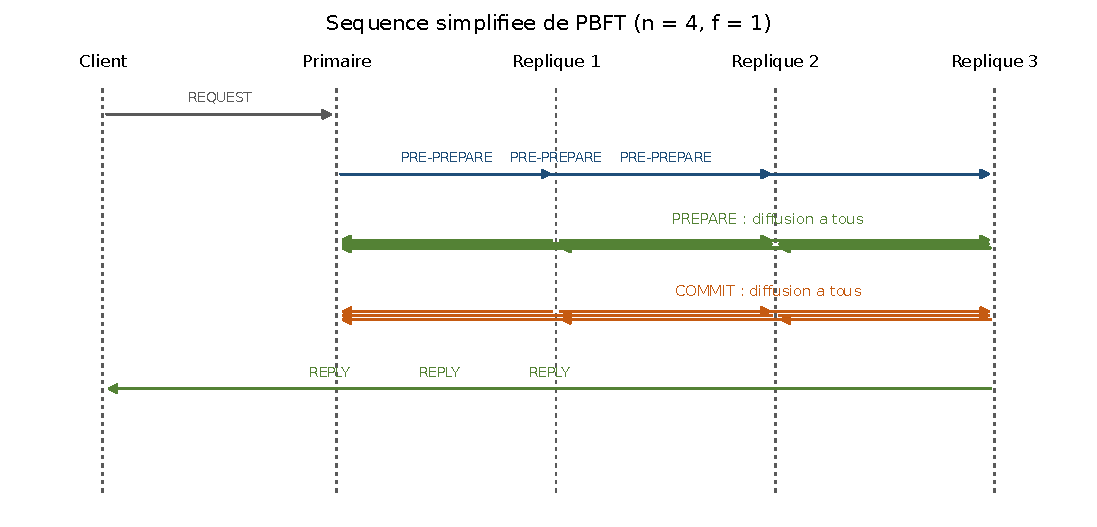
\includegraphics[width=0.82\textwidth]{fig2_phases_pbft.pdf}
  \end{center}
  \vspace{-0.2cm}
  \small
  Le primaire propose ; les répliques préparent puis confirment ; le client reçoit
  $f+1$ réponses identiques. Le coût est en $O(n^2)$ messages par décision.
\end{frame}

\begin{frame}{CometBFT : ce que nous mesurons réellement}
  \begin{columns}[T,onlytextwidth]
    \begin{column}{0.56\textwidth}
      \begin{enumerate}
        \item Un validateur propose un bloc.
        \item Les validateurs diffusent un \emph{prevote}.
        \item Après $2f+1$ prevotes, ils diffusent un \emph{precommit}.
        \item Après $2f+1$ precommits, le bloc est \textbf{final} : pas de fork probabiliste.
      \end{enumerate}
      \vspace{0.2cm}
      \small
      Le \texttt{timeout\_commit} vaut 1 s dans notre configuration : la latence
      observée inclut ce délai incompressible.
    \end{column}
    \begin{column}{0.40\textwidth}
      \begin{block}{Conséquence pratique}
        \small
        La finalité est immédiate, mais la progression dépend d'un quorum.
        Si les validateurs honnêtes restants sont moins de $2f+1$, la chaîne
        s'arrête : la sûreté tient, la vivacité non.
      \end{block}
      \begin{block}{Application}
        \small
        Une transaction porte l'empreinte d'un diplôme ; les universités
        comparent la valeur à leurs propres registres.
      \end{block}
    \end{column}
  \end{columns}
\end{frame}

\begin{frame}{Banc d'essai et scénarios}
  \begin{columns}[T,onlytextwidth]
    \begin{column}{0.50\textwidth}
      \small
      \begin{itemize}
        \item CometBFT v0.38.17, application \texttt{kvstore}, Docker.
        \item 4, 7 puis 10 validateurs ; une machine, 10 Go de RAM.
        \item Retards aller simple injectés par \texttt{tc netem} : 10 à 45 ms (Dakar, Saint-Louis, Ouagadougou, Abidjan, Bamako, Niamey, Lomé, Cotonou, Bissau, Ziguinchor).
        \item Charge : 20 envois séquentiels pour la latence, 200 transactions avec 20 envois simultanés pour le débit.
        \item 3 essais indépendants par scénario.
      \end{itemize}
    \end{column}
    \begin{column}{0.46\textwidth}
      \begin{tabular}{@{}lll@{}}
        \toprule
        Scénario & Configuration & But \\
        \midrule
        S1 & 4, sans retard & référence \\
        S2 & 4, retard UEMOA & effet réseau \\
        S3 & 7 et 10, retard & passage à l'échelle \\
        S4 & 4, $f$ puis $f+1$ & pannes, reprise \\
        \bottomrule
      \end{tabular}
      \vspace{0.3cm}
      \begin{alertblock}{Limite annoncée}
        \small
        Nous provoquons des \textbf{pannes franches} (\texttt{docker stop}), pas
        des validateurs qui mentent activement.
      \end{alertblock}
    \end{column}
  \end{columns}
\end{frame}

\begin{frame}{Résultats : la latence reste de l'ordre de la seconde}
  \begin{center}
    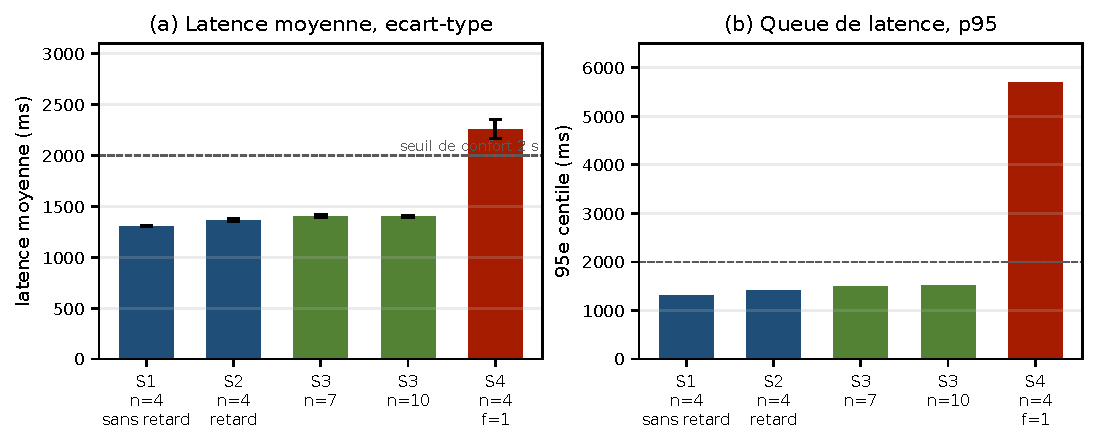
\includegraphics[width=0.95\textwidth]{fig3_latence.pdf}
  \end{center}
  \vspace{-0.1cm}
  \small
  \begin{itemize}
    \item S1 : 1\,303 ms $\pm$ 9 ms ; S2 : 1\,365 ms $\pm$ 27 ms ; S3 à 7 et 10 : 1\,403 et 1\,401 ms.
    \item Avec $f=1$ panne : moyenne 2\,258 ms, p95 5\,698 ms. La queue explose, pas la médiane.
  \end{itemize}
\end{frame}

\begin{frame}{Résultats : le débit baisse peu, puis s'effondre en panne}
  \begin{columns}[T,onlytextwidth]
    \begin{column}{0.54\textwidth}
      \begin{center}
        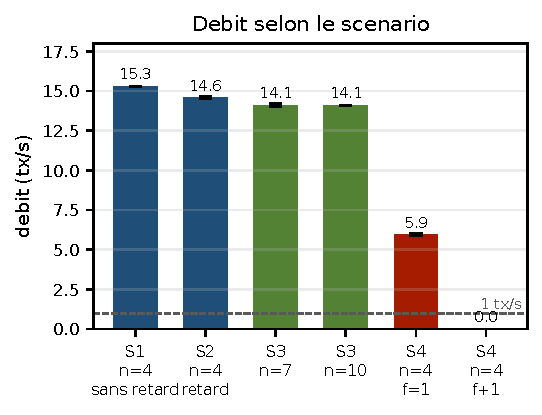
\includegraphics[width=\textwidth]{fig4_debit.pdf}
      \end{center}
    \end{column}
    \begin{column}{0.42\textwidth}
      \small
      \begin{itemize}
        \item 15,3 tx/s à 4 nœuds sans retard.
        \item 14,6 tx/s avec retard ; 14,1 tx/s à 7 et 10 nœuds.
        \item Avec $f=1$ panne : 5,9 tx/s.
        \item Avec $f+1=2$ pannes : 0 tx/s, chaîne bloquée.
      \end{itemize}
      \begin{block}{Lecture}
        \small
        Le passage de 4 à 10 validateurs coûte environ 7,5 \% de latence et
        7,8 \% de débit. Le seuil de 1 tx/s reste tenu, sauf quand le quorum
        n'est plus atteignable.
      \end{block}
    \end{column}
  \end{columns}
\end{frame}

\begin{frame}{Pannes : la sûreté tient, la vivacité s'arrête}
  \begin{center}
    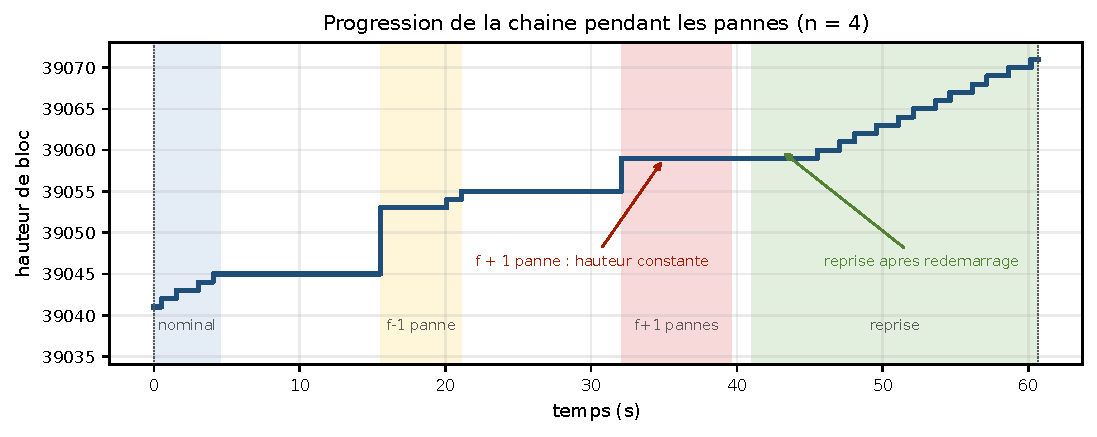
\includegraphics[width=0.92\textwidth]{fig5_pannes.pdf}
  \end{center}
  \vspace{-0.1cm}
  \small
  \begin{itemize}
    \item $f=1$ panne : la hauteur continue d'avancer, aucune bifurcation.
    \item $f+1=2$ pannes : la hauteur reste constante, les transactions échouent.
    \item Après redémarrage : premier nouveau bloc après 8,6 s, sans rollback visible.
  \end{itemize}
\end{frame}

\begin{frame}{Le coût caché : les messages augmentent en $O(n^2)$}
  \begin{columns}[T,onlytextwidth]
    \begin{column}{0.48\textwidth}
      \begin{center}
        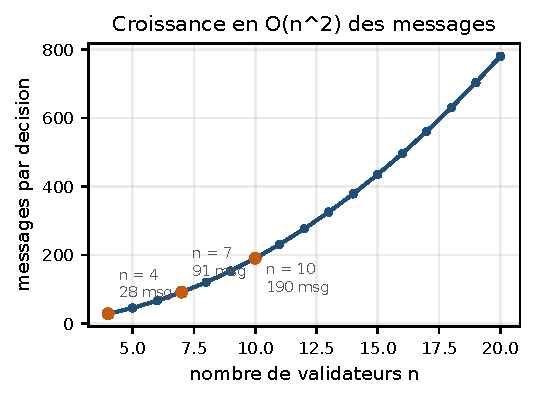
\includegraphics[width=\textwidth]{fig6_messages.pdf}
      \end{center}
    \end{column}
    \begin{column}{0.48\textwidth}
      \begin{tabular}{@{}rrrr@{}}
        \toprule
        $n$ & $f$ & Quorum & Messages \\
        \midrule
        4 & 1 & 3 & 28 \\
        7 & 2 & 5 & 91 \\
        10 & 3 & 7 & 190 \\
        \bottomrule
      \end{tabular}
      \vspace{0.3cm}
      \small
      \begin{itemize}
        \item Formule PBFT : $2n^2 - n$ messages par décision.
        \item De 4 à 10 validateurs, le coût est multiplié par 6,8.
        \item Dans notre banc, le \texttt{timeout\_commit} et le client dominent encore : le coût réseau n'est pas le facteur limitant à cette échelle.
      \end{itemize}
    \end{column}
  \end{columns}
\end{frame}

\begin{frame}{Discussion : ce que le consensus garantit, et ce qu'il ne garantit pas}
  \begin{columns}[T,onlytextwidth]
    \begin{column}{0.48\textwidth}
      \begin{block}{Ce qui est garanti}
        \small
        \begin{itemize}
          \item Accord sur l'ordre des blocs tant que $n \geq 3f+1$.
          \item Finalité immédiate : un bloc validé n'est pas réorganisé.
          \item Reprise après redémarrage des validateurs.
        \end{itemize}
      \end{block}
    \end{column}
    \begin{column}{0.48\textwidth}
      \begin{block}{Ce qui n'est pas garanti}
        \small
        \begin{itemize}
          \item La \textbf{véracité} du diplôme : un consensus peut valider une fausse empreinte.
          \item La vivacité si plus de $f$ validateurs sont indisponibles.
          \item La résistance à un validateur qui ment : non testée expérimentalement.
        \end{itemize}
      \end{block}
    \end{column}
  \end{columns}
  \vspace{0.2cm}
  \small
  \textbf{Gouvernance :} qui admet une université, qui révoque une clé, que faire
  d'un diplôme dont l'émetteur conteste l'inscription ? Le code ne répond pas à
  ces questions ; le consortium doit le faire.
\end{frame}

\begin{frame}{Conclusion}
  \begin{block}{Réponse à la question}
    \small
    Pour un consortium de 4 à 10 universités, CometBFT offre une finalité de
    l'ordre de 1,3 à 1,5 s et un débit de 14 à 15 tx/s, compatible avec la
    vérification de diplômes. La cohérence tient sous $f$ pannes ; elle s'arrête
    dès $f+1$ pannes, sans divergence. La tolérance byzantine reste une garantie
    théorique dans notre banc.
  \end{block}
  \begin{columns}[T,onlytextwidth]
    \begin{column}{0.48\textwidth}
      \small
      \textbf{À retenir}
      \begin{itemize}
        \item BFT = sûreté sous faute byzantine, pas véracité des données.
        \item Le quorum est le cœur : $2f+1$ sur $3f+1$.
        \item La panne est le premier risque opérationnel.
      \end{itemize}
    \end{column}
    \begin{column}{0.48\textwidth}
      \small
      \textbf{Perspectives}
      \begin{itemize}
        \item Tester un validateur byzantin actif.
        \item Mesurer les latences réelles entre capitales.
        \item Ajouter la révocation et la gouvernance des clés.
      \end{itemize}
    \end{column}
  \end{columns}
  \vspace{0.25cm}
  \centering
  \textbf{Merci. Questions ?}\\[0.1cm]
  \footnotesize
  Discutants : groupe 7 \quad\textbullet\quad Rapporteurs : groupe 2 \quad\textbullet\quad Dépôt : \texttt{rendu\_final\_groupe3}
\end{frame}

\end{document}
